\chapter{Grundlagen}
\label{cha:Fundamentals}

\section{AR.Drone 2.0}
%Christoph
Bei der AR.Drone 2.0 handelt es sich um einen ferngesteuerten Quadrocopter des französischem Herstellers Parrot SA. \cite{drone} Die Drohne ist standardmäßig steuerbar mit einer mobilen Applikation für Android und iOS Geräte. Dafür baut sie ein WLAN Netzwerk auf, mit dem sich die Geräte verbinden können. Zur Steuerung stellt die AR.Drone ein Interface zur Verfügung, mit dem sie ferngesteuert werden kann. \newline
Im Umfang der Studienarbeit wird die aktuellste Version der AR.Drone 2.0 verwendet. Diese zeichnet sich unter Anderem durch eine Frontkamera mit einer Auflösung von 1280×720 Pixeln und einer Bildrate von 30 fps aus. Weiterhin ist Sie mit einer zum Boden gerichteten QVGA Kamera ausgerüstet, welche 60 Bilder pro Sekunde aufnimmt. \newline
Die Drohne orientiert sich beim Fliegen mit Hilfe einer Vielzahl von Sensoren. Dazu gehören ein dreiachsiges Gyroskop und ein Magnetometer. Weiterhin nutzt sie Beschleunigungs-, Ultraschall- und Luftdrucksensoren. \newline
Der Grund für die Wahl der Drohne ist vor allem der vergleichsweise niedrige Preis von ca. 200€ und der starken Verbreitung in der Forschung. Dadurch gibt es bereits eine Vielzahl von Projekten, die dazu führen, dass die Drohne und das dazugehörige Interface zu einem großen Umfang fehlerfrei funktionieren. \newline
Weiterhin gibt es schon ROS Nodes (siehe \ref{ROS}) und konfigurierte Modelle in Simulationsumgebungen, welche die Arbeit an dem Projekt beschleunigen.


\section{ROS}
%Max
\label{ROS}
\subsection{Allgemeines}
Das Robotic Operating System, kurz ROS, ist eine Sammlung von Softwareframeworks für die Entwicklung von Software für persönliche Roboter. Es stellt entsprechende Bibliotheken und Werkzeuge zur Verfügung, um Entwicklern die Programmierung zu vereinfachen. Dabei bietet ROS einem Betriebssystem ähnliche Funktionalitäten auf Basis eines homogenen Computercluster. Dazu gehören Hardwareabstraktion, low-level Steuerung, Nachrichtevermittlung zwischen verschiedenen Prozessen und Paketmanagement. Trotz der Notwendigkeit hoher Reaktivität und geringer Latenz bei der Steuerung von Robotern handelt es sich es de facto nicht um ein richtiges Betriebssystem , obwohl es durch den Namen(\grqq Operating System\grqq) suggeriert wird. Dennoch ist es möglich Echtzeitcode (\grqq realtime code\grqq) in ROS zu integieren \cite{realtimecode}. ROS ist eins der am meisten genutzten Frameworks und hat eine stark wachsende Gemeinschaft, was es in Kombination mit dessen Feature zu einer enorm wichtigen Technologie macht.

\subsection{ROS Nodes}
ROS baut auf einem einfachen Konzept auf, dem Publish-Subscribe Pattern, bei welchem ein Publisher ein Nachricht mit einem festem Thema verschicken kann und ein beliebiger Subscriber, der sich für das Thema interessiert, ist in der Lage diese zu empfangen, zu verarbeiten und unter Umständen erneut zu versenden.  Somit besteht eine ROS Anwendung aus der Regel aus vielen kleinen Teilen, den sogenannte Nodes. Jede Node hat ihre eigenen Aufgabe und registriert sich auf ein bestimmtes Thema(Topic), verarbeitet die empfangen Daten und publiziert sie für andere Nodes. Somit kann eine Node sowohl Publisher, als auch Subscriber sein. Topics werden in ROS durch einen festen Nachrichtentyp definiert. Dessen exakter Aufbau muss vor Verwendung deklariert werden um einen einheitlichen Nachrichtenaustausch zu gewähren. Wie in der Abbildung unterhalb zu sehen, wird der Nachrichtentransfer durch eine zentrale Einheit geregelt, sodass Daten wirklich nur die Nodes erreichen, die sich auch dafür interessieren. Dieser zentrale Bestandteil ist in ROS der Roscore, bei welchem sich alle Nodes zur Erstellung registrieren. Sozusagen eine Masternode, welche sich um die Verwaltung der anderen Nodes kümmert. Im Unterschied zum Pattern kümmert sich der Roscore nur um die anfängliche Vermittlung der Nodes untereinander. %TODO nicht Sicher
\begin{figure}[ht]
		\centering
	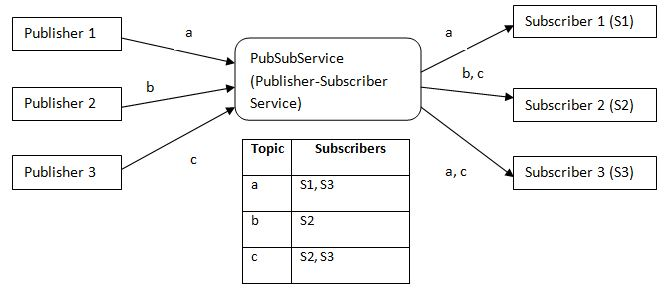
\includegraphics[scale=0.7]{Bilder/pubsub1.jpg}
	\caption[Publish-Subscribe Pattern]{Publish-Subscribe Pattern}

\end{figure}
\newline
ROS Nodes können in verschiedenen Sprachen implementiert werden, da die Kommunikation über die festen Nachrichtentypen geschieht, welche über den Roscore ausgetauscht werden. Dadurch ist es möglich Nodes in C++, Python und ebenfalls Lisp zu programmieren. Wodurch das ganze Konzept enorm flexibel gestaltet wird. Die fest definierten Nachrichtentypen verhindern, dass es an den Schnittstellen zu Problemen kommt und Nachrichten von allen Nodes einheitlich empfangen und versendet werden. \newline
Durch diese Modularität ist einfacher Komponenten und Funktionalitäten sowohl zu verwalten, als auch zu warten. Ebenfalls sind durch einheitliche Schnittstellen der Austausch von Nodes einfach und ermöglicht ein flexibles Ökosystem.


\section{Simulation}
Da es besonders beim Flug von Quadrocoptern schnell zu Schäden kommen kann und das sowohl  in langen Ausfallzeiten, als auch zu erhöhten Materialkosten führen. Speziell beim Test von autonomen Verhalten ist der Test der Features in realer Umgebung somit mit hohem Risiko verbunden. Um dies zu vermeiden ist die Simulation von Quadrocoptern und verschiedener Umgebungen unabdingbar. Ebenfalls erleichtert eine simulierte Version der Drohne die Entwicklung, da sie nicht immer physikalisch vorhanden sein muss. Dabei ist es allerdings notwendig, insbesondere bei Bilddaten, dass die reale Situation möglichst realitätsnah abgebildet wird, sodass das Verhalten im realen Umfeld entsprechend ähnlich ist. \newline
Durch die Integration von ROS kommt die Simulationsumgebung Gazebo als Bestandteil mit. Anfänglich handelte es sich um ein ROS Paket, mittlerweile ist es allerdings ein eigenständiges Ubuntupaket und benötigt de facto kein ROS.
%Max

\section{Fuzzylogik}
%Würde erwähnen dass wir es verwenden
%wollen wir das überhaupt reinnehmen? haben wir ja eigentlich gar nicht gemacht und mussten wir uns auch %null mit beschäftigen


\section{Kinect}
%Max